\receta{Marranitas}

Rinde 18 Unidades.

\begin{ingredientes}
\item 9 Plátanos Maduros
\item 1.5 kg Tocino
\item 1 L Aceite 
\end{ingredientes}
\preparacion

Se cortan el tocino en cubos pequeños y se fritan para obtener chicharrones. Por aparte se fríen troncos de medio plátano hasta que queden ligeramente dorados. Los troncos se pisan hasta obtener un masa que permita armar arepitas.\\

Se hacen arepitas y se les pone encima los cubitos de chicharrón fritos, y con la masa se encierran los chicharrones formando bolitas las cuales de ponen nuevamente en la olla de freír hasta que doren levemente.\\
%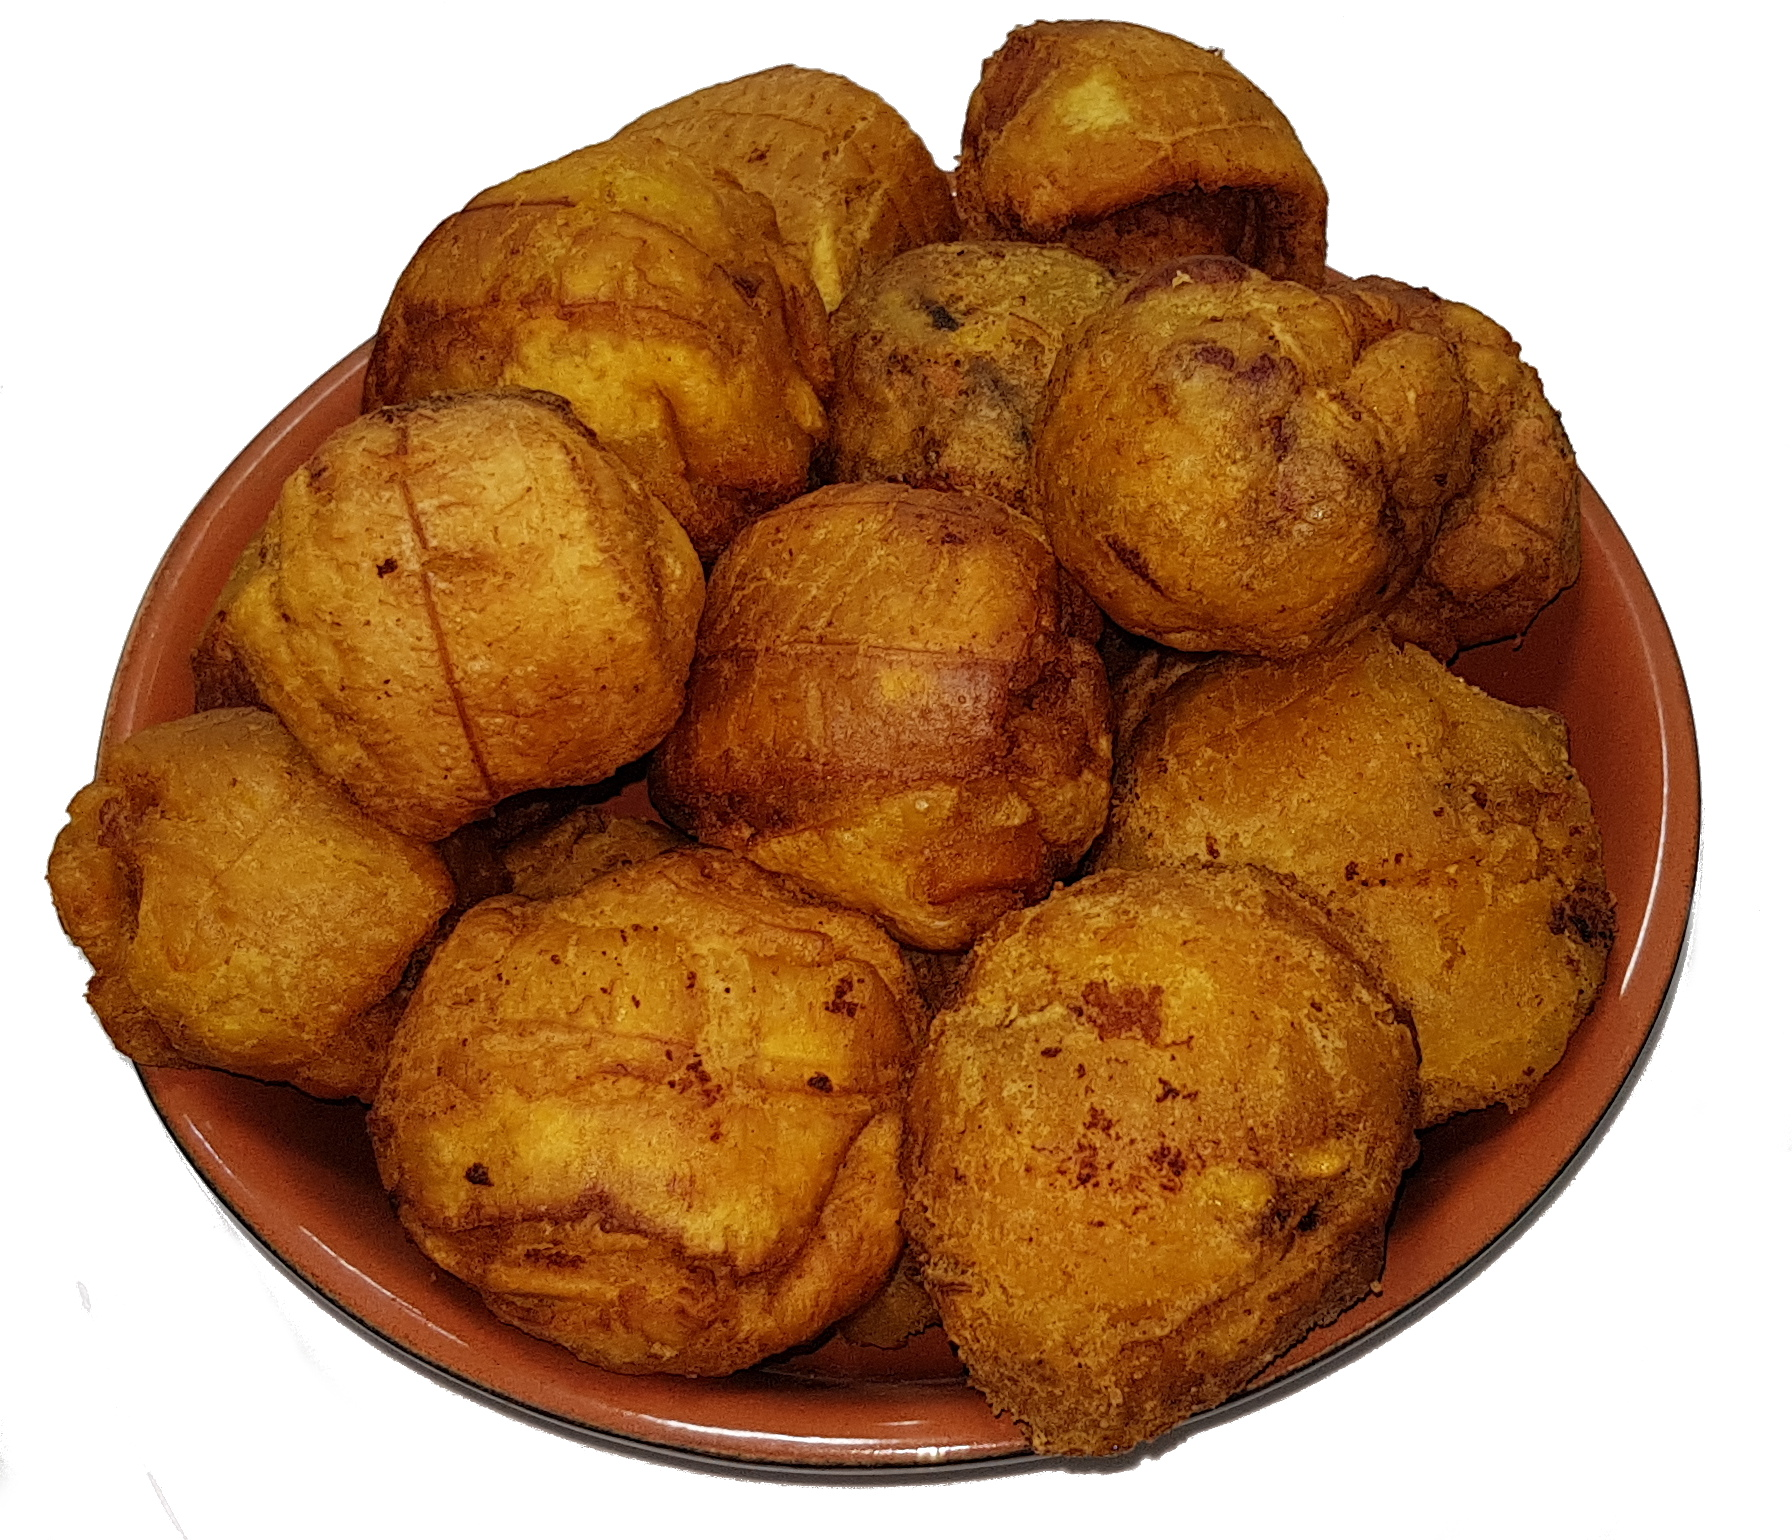
\includegraphics[width=0.8\textwidth]{fotos/marranitas}